\graphicspath{{./assets/}}
\setcounter{mtc}{9}
\chapter{7th Sprint : CI/CD Workflows }
\fancyhead[R]{\ungaramond\small\textbf{Chapter IX.  7th Sprint: CI/CD Workflows   }}

\minitoc

\section*{Introduction}
CI/CD workflows are a set of automated processes that enable us to continuously build, test, and deploy software changes. These workflows help to speed up the software development process by enabling developers to quickly detect and fix issues, and to release new software versions frequently and reliably. 


\section{Sprint backlog :}

\begin{longtable}[H]{|m{1.5cm}|m{3cm}|m{1.5cm}|m{9cm}|}
\hline
{\textbf{Epic ID}} & {\textbf{Epic}} & {\textbf{Story ID}} & {\textbf{Story}}\\
\hline
1  & Setting up a GitOPS compliant CI/CD workflow for the applications in development.  &  1.1	 & Setting up the CI/CD orchestrator.\\
\cline{3-4}
& & 1.2 & SCM restructuring and code adaptation. \\
\cline{3-4}
& & 1.3	& Preparing container images for the different workloads in development.  \\
\cline{3-4}
& & 1.4	& Developing GitOPS oriented pipelines for the build, scan, and deliver phases in the various environments.  \\
\cline{3-4}
\hline
\caption{7th Sprint Backlog}
\end{longtable}

\section{UML Design: Activity diagram for the CI/CD workflows } 

In the previous chapter, various CI/CD tools have been self-hosted in a complementary manner. Taking advantage of these tools, we are aiming to provide a reliable workflow to funnel the developed workloads through the various steps of code analysis, containerized artifact building, and deployment in various environments.  

 

The following is an activity diagram underlining the various interfaces, actors, and actions of these processes: 

\begin{figure}[H]\centering
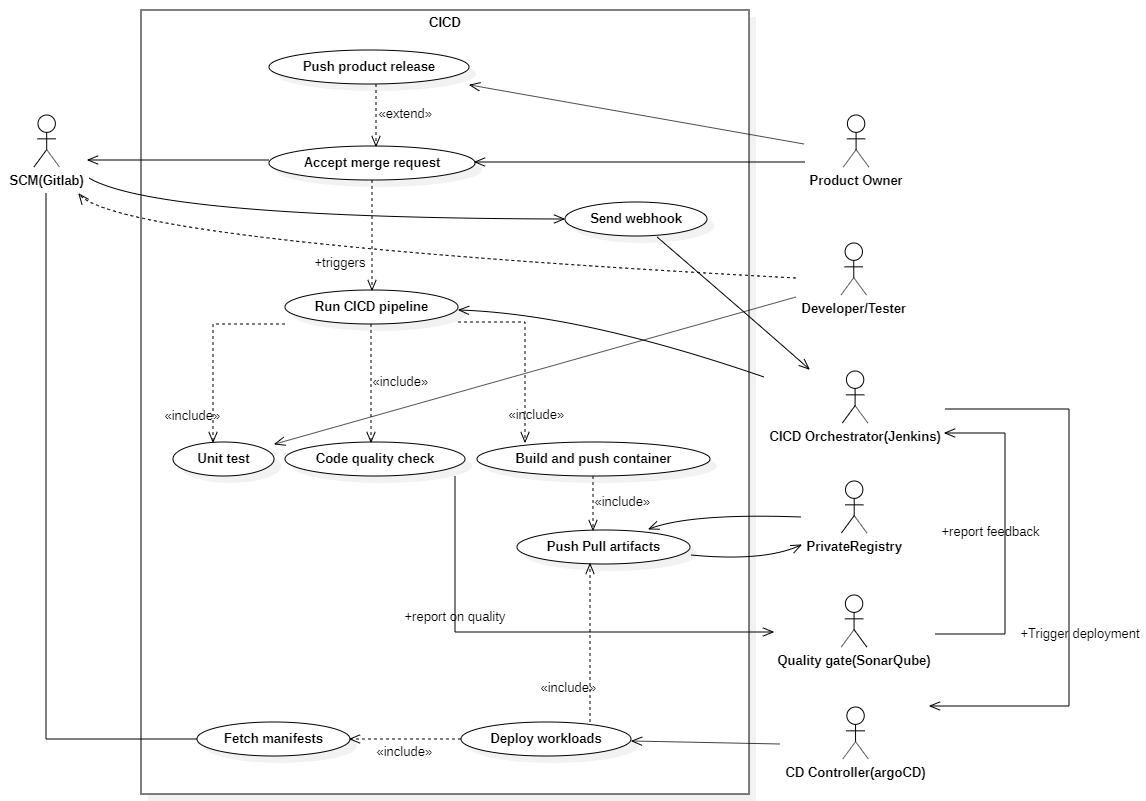
\includegraphics[width=1.0\textwidth,angle=00]{assets/f45.png}
\caption{ Activity diagram for the CI/CD workflows}
\label{fig:Activity diagram for the CI/CD workflows}
\end{figure}

\section{UML Design: Sequence diagram of the CI/CD workflow }

Next, let’s look at the sequence diagram for the CI/CD workflow: 
\begin{figure}[H]\centering
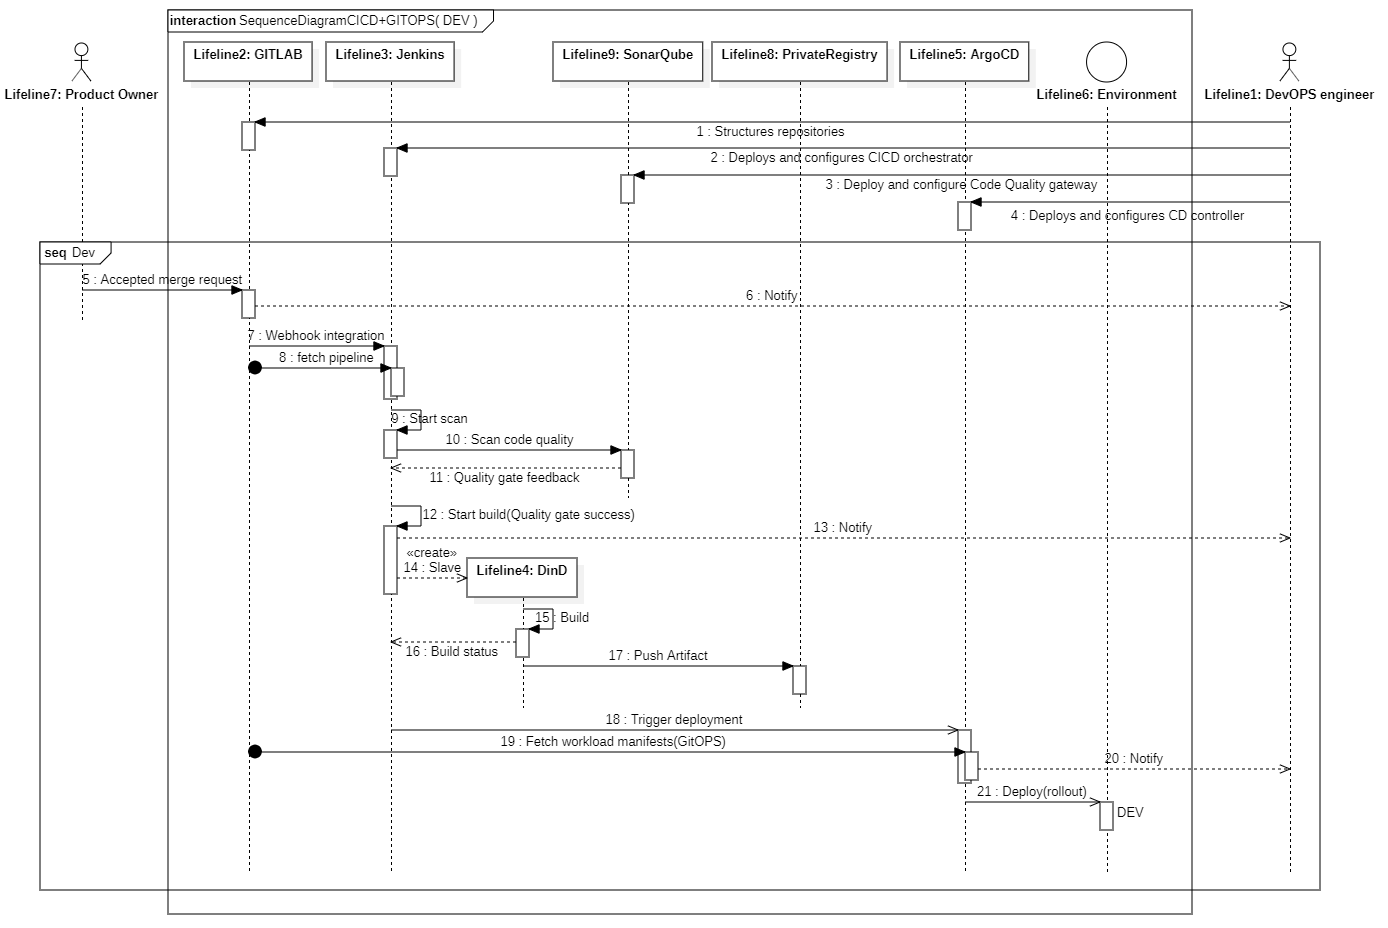
\includegraphics[width=1.0\textwidth,angle=00]{assets/f46.png}
\caption{ Sequence diagram of the CI/CD workflow}
\label{fig:sequence diagram of the CI/CD workflow}
\end{figure}

\section{CI/CD workflow steps }

\subsection{Architecture of the software under development }

Among the proprietary software developed by the company, we have “SYSTNAPS” which is used for data processing by a few well known companies such as “Dassault-Systems” and others. It is mainly composed of three major parts as shown in the diagram below : 

\begin{figure}[H]\centering
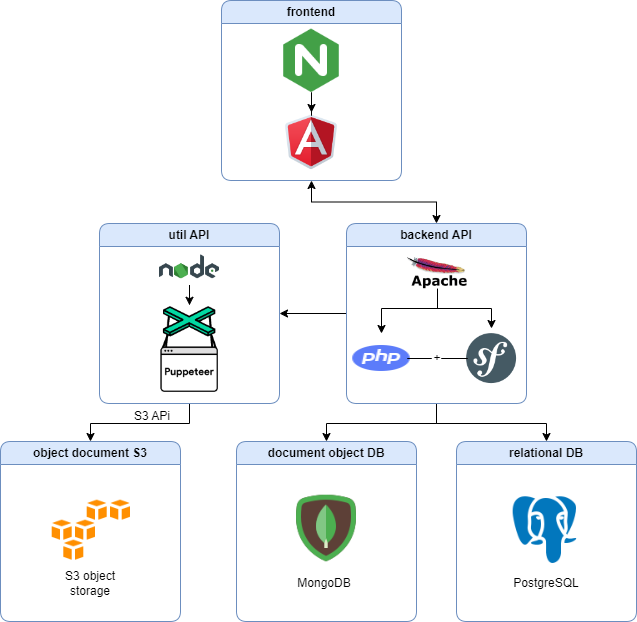
\includegraphics[width=1.0\textwidth,angle=00]{assets/f47.png}
\caption{Architecture of the software under development}
\label{fig:Architecture of the software under development}
\end{figure}

The backend api interacts with the frontend by providing the implemented computing functions. It also uses a utility api which uses puppeteer and various other libraries for graph rendering. Both relational and document databases are used for data storage. Some of the data is stored in document format in an S3 compatible storage backend.

\subsection{Containerizing artifacts:}

Container images for the application components are built inside the docker in docker instance we have previously build. It is configured to be able to authenticate with the private registry to pull the base image and push the resulting artifact. 

\subsubsection{Dockerfile of the backend API container image }

For building the container image for the backend api, we first build a base image which contains most of the packages and immutable config. 

The resulting dockerfile for the actual container image is as follows: 

\begin{listing}[H]
    \inputminted[firstline=1,lastline=30]{Dockerfile}{codeListing/syst_backend_Dockerfile}
\end{listing}
\begin{listing}[H]
     \inputminted[firstline=31]{Dockerfile}{codeListing/syst_backend_Dockerfile}
    \caption{Backend API Dockerfile}
    \label{lst:API Dockerfile}
\end{listing}
 

\subsubsection{Dockerfile of the frontend container image }

As with the backend part, this image is built from a base that contains all that is immutable. Building the frontend part of the application is done in two stages as follows: 

 \begin{listing}[H]
    \inputminted{Dockerfile}{codeListing/syst_frontend_Dockerfile}
    \caption{Frontend Dockerfile}
    \label{lst:Dind Dockerfile}
\end{listing}

\subsubsection{Dockerfile of the utility API container image} 

 
\subsection{Code quality }

\subsubsection{Conceptual design }

To ensure code quality, the first step is to scan the developed code of both the frontend, backend and utility for vulnerabilities and other irregularities.  

A quality gate is then used to inform the cicd orchestrator of the level of stability. The following diagram showcases the involved processes of this stage: 

\begin{figure}[H]\centering
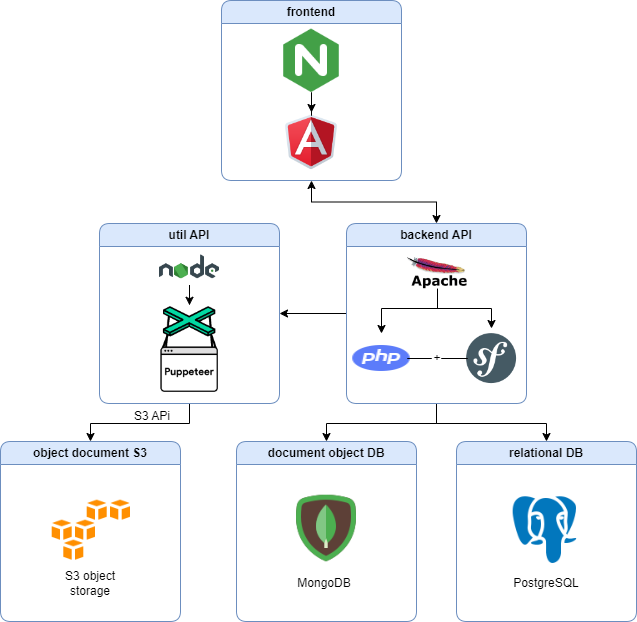
\includegraphics[width=1.0\textwidth,angle=00]{assets/f47.png}
\caption{ Conceptual design of Code quality }
\label{fig:conceptual design of Code quality }
\end{figure}


\subsubsection{Implementation }

As illustrated in this figure, the code scanning process is initiated by our orchestrator following each accepted merge request in the SCM. The following is the pipeline for the scan job: 

 
\begin{listing}[H]
    \inputminted{Dockerfile}{codeListing/Jenkinsfile_scan}
    \caption{ Jenkins file scan}
    \label{lst:jenkinsfile_scan}
\end{listing}
 

\subsection{Building artifacts: }

\subsubsection{Conceptual design :}

Containerizing the applications contributes to portability, consistency, and resource efficiency of the workloads to be deployed. Following each approved merge request, a build step is processed. 

The following diagram illustrates this process and the interaction between the key components: 

\begin{figure}[H]\centering
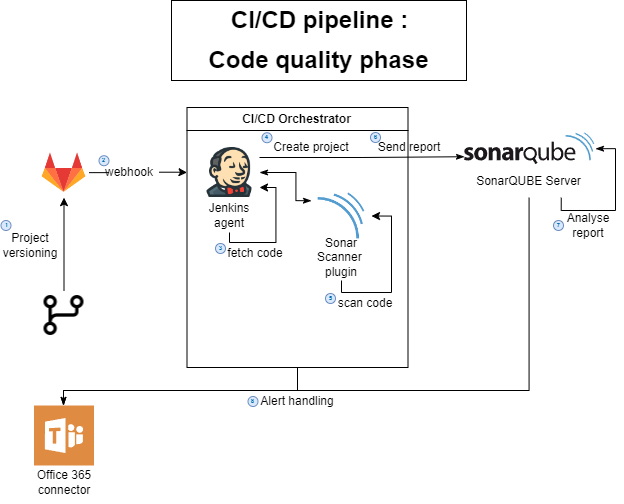
\includegraphics[width=1.0\textwidth,angle=00]{assets/f48.png}
\caption{Conceptual design of building artifact }
\label{fig:Conceptual design of building artifact }
\end{figure}

\subsubsection{Implementation :}

In similar fashion to the code scanning step, building artifacts is initiated following each approved merge request. A webhook is sent by the SCM tool to Jenkins which starts the job using the following pipeline: 

\begin{listing}[H]
    \inputminted[firstline=1,lastline=40]{Dockerfile}{codeListing/Jenkinsfile_build}
\end{listing}

\begin{listing}[H]
    \inputminted[firstline=41,lastline=75]{Dockerfile}{codeListing/Jenkinsfile_build}
\end{listing}

\begin{listing}[H]
    \inputminted[firstline=76]{Dockerfile}{codeListing/Jenkinsfile_build}
    \caption{Jenkins build}
    \label{lst:jenkinsfile_build}
\end{listing}

The build and publish steps are processed in a DinD agent spun inside the Kubernetes cluster. The agent is provided with the necessary credentials to authenticate with the private registry as well as a persistent volume in which it stores the cache data of image layers. 

For each build process, the name and tag of the image are programmatically extracted both from the respective repository name in the SCM and the release tag. 

 

\subsection{Delivering artifacts }

\subsubsection{Conceptual design:}

For delivering artifacts, the CI/CD orchestrator, Jenkins, is used in conjunction with argocd, our CD/CD controller. ArgoCD uses deployment manifests pushed to the SCM in order to create the workload objects. 

The product delivery process is initiated in any of these cases depending on the rollout strategy: 

\begin{itemize}[label={--}]
\item A release tag is pushed to the SCM. 
\item A newer container image with the same tag is pushed to \item the private registry. 
\end{itemize}

An update to the manifests is pushed to the SCM. 

The following is a general diagram of the delivery process: 

\begin{figure}[H]\centering
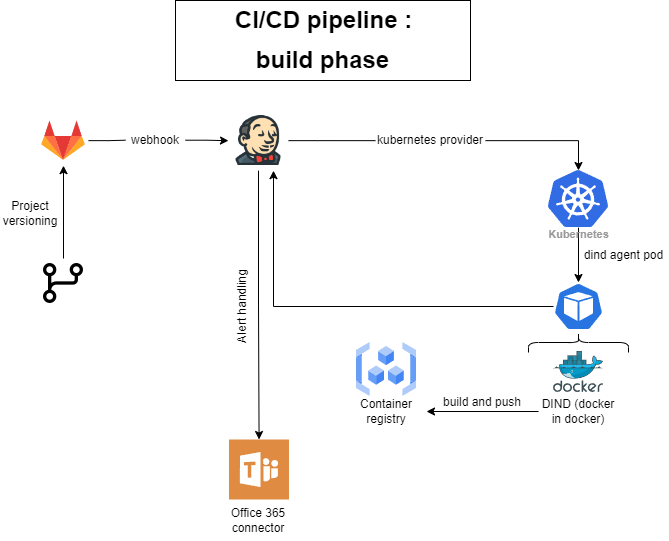
\includegraphics[width=1.0\textwidth,angle=00]{assets/f49.png}
\caption{Conceptual design of Delivering artifacts }
\label{fig:Conceptual design of Delivering artifacts }
\end{figure}

\subsubsection{Implementation: }

The deployment manifests, configmaps, secrets, ingressroutes and other Kubernetes objects needed for deploying the applications are templated with each delivery using ytt. This makes the container configuration reusable and extensible.  


\paragraph{Overview: }

The following is an overview of the declarative Jenkinsfile used : 

 
\begin{listing}[H]
    \inputminted[firstline=1,lastline=30]{Dockerfile}{codeListing/Jenkinsfile_deploy_overview}
\end{listing}
 
\begin{listing}[H]
    \inputminted[firstline=31]{Dockerfile}{codeListing/Jenkinsfile_deploy_overview}
    \caption{jenkins deploy overview}
    \label{lst:jenkinsfile_deploy_overview}
\end{listing}

\paragraph{Templating manifests: }

Using ytt from Carvel, we are able to create Kubernetes manifests in the YAML format using a specific variable schema. As shown in the stage below, reusable templates are first pulled from the SCM, templated using ytt, and then pushed to an SCM repository in a secure manner: 

 \begin{listing}[H]
    \inputminted[firstline=1,lastline=15]{Dockerfile}{codeListing/Jenkinsfile_deploy_templating}
\end{listing}

 \begin{listing}[H]
    \inputminted[firstline=16,lastline=49]{Dockerfile}{codeListing/Jenkinsfile_deploy_templating}
\end{listing}

 \begin{listing}[H]
    \inputminted[firstline=50]{Dockerfile}{codeListing/Jenkinsfile_deploy_templating}
    \caption{Jenkins deploy templating}
    \label{lst:jenkinsfile_deploy_templating}
\end{listing}


 
\paragraph{Delivering workloads: }

Once the deployment manifests are present in the SCM repository, Jenkins then informs argocd to begin the delivery process. The following is the declarative stage used: 

\begin{listing}[H]
    \inputminted[firstline=1,lastline=10]{Dockerfile}{codeListing/Jenkinsfile_deploy_delivery}
\end{listing}

\begin{listing}[H]
    \inputminted[firstline=11,lastline=45]{Dockerfile}{codeListing/Jenkinsfile_deploy_delivery}
\end{listing}

\begin{listing}[H]
    \inputminted[firstline=46]{Dockerfile}{codeListing/Jenkinsfile_deploy_delivery}
    \caption{Jenkins deploy delivery}
    \label{lst:jenkinsfile_deploy_delivery}
\end{listing}

\section*{Conclusion}
In conclusion, implementing a CI/CD workflow in Kubernetes is a complex but rewarding process that requires a combination of different tools and techniques. 

Jenkins serves as the main orchestrator for the CI/CD process, with DinD agents building container images, and Gitlab as the source code management tool. 

The use of ArgoCD as the CD controller, along with Harbor for storing container images, provides a streamlined approach for deploying applications. 

SonarQUBE helps in identifying code issues early in the development process. 

Additionally, the use of templating techniques such as ytt and jinja2 allows for efficient and consistent deployment of applications across different environments.  

Overall, the implementation of a robust CI/CD pipeline in Kubernetes helps in achieving faster and more reliable application delivery.